\documentclass[12pt,a4paper]{article}%шаблон для статьи, шрифт 12 пт
\usepackage[utf8x]{inputenc} %использование кодировки Юникод UTF-8
\usepackage[russian]{babel} %пакет поддержки русского языка
\usepackage{lipsum}%Рыба-текст
\usepackage[compact]{titlesec}%для titlespacing
\titlespacing*{\section}{0.75cm}{1em}{0.1em}%отступ заголовка
%\titlespacing{\заголовок}{слева}{перед}{после}[справа]
\titlespacing*{\subsection}{0.75cm}{1em}{0.1em}
\usepackage{indentfirst}%отступ первого абзаца
\setlength{\parindent}{0.75cm}
\usepackage[labelsep=endash]{caption}%тире вместо двоеточия в картинках
\usepackage{graphicx}%кртинки
\usepackage{comment}%комментарии
\usepackage{tabularx}%таблицы
\usepackage{amsmath}
\usepackage{amssymb}


%перенос строк внутри таблиц
\newcommand{\specialcell}[2][c]{%
	\begin{tabular}[#1]{@{}c@{}}#2\end{tabular}}

\usepackage[labelsep=endash]{caption} %тире вместо двоеточия в названиях 
%\renewcommand\thefigure{\arabic{section}.\arabic{figure}}
%\renewcommand{\labelenumii}{\arabic{enumi}.\arabic{enumii}.} % Сквозная нумерация

\begin{document}

\thispagestyle{empty}

\begin{center}
\Large{
	\textbf{МИНОБРНАУКИ РОССИИ}
	
	\textbf{Санкт-Петербургский государственный}
	
	\textbf{электротехнический университет «ЛЭТИ»}
	
	\textbf{им. В.И. Ульянова (Ленина)}
	
	\textbf{Кафедра Физики}
}
\end{center}

\topskip=0pt
\vspace*{\fill}
\begin{center}
\Large{
	\textbf{
		ЛАБОРАТОРНАЯ РАБОТА №3(2)\\
		по дисциплине «Физика»\\
		Тема: Исследование динамики свободных гармонических колебаний в поле силы тяжести\\
	}
}
\end{center}
\vspace*{\fill}

\begin{tabular}{lcr}
Студент гр. 9892 & \begin{tabular}{p{60mm}} \\ \hline \end{tabular} & Лескин К.А.  \\\\
Преподаватель    & \begin{tabular}{p{60mm}} \\ \hline \end{tabular} & Чурганова С.С. \\\\
\end{tabular} 

\begin{center}
Санкт-Петербург\\
2020
\end{center}
%////////////////////////////////////////////////////////////////////////////////////////////////
%////////////////////////////////////////////////////////////////////////////////////////////////
%////////////////////////////////////////////////////////////////////////////////////////////////
\newpage

\section*{Цель работы}
Изучение закономерностей колеба-
тельного движения тела в однородном поле силы тяжести;
исследование процессов превращения энергии в консерва-
тивных системах; определение момента инерции физиче-
ского маятника.

\section*{Приборы и принадлежности}
Физический маятник;
секундомер; масштабная линейка, чертежный треугольник.

Конструкция оборотного маятника представлена на
рис. \ref{1}. На стержне 1 закреплены два диска – D 1 и D 2. 
Маятник может быть подвешен на кронштейне к легкой
призме, трение в которой пренебрежимо мало.

\begin{figure}[h!]
	\centering
	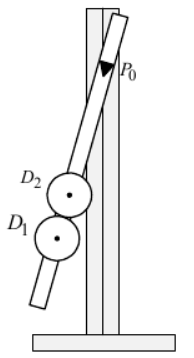
\includegraphics[width=0.5\linewidth]{pic/1}
	\caption{}
	\label{1}
\end{figure}

\newpage

\section*{Основные исследуемые закономерности}

Физическим маятником называют тело с распределенной массой (систему
тел), ось вращения которого расположена выше центра масс маятника. 
Период колебаний такого маятника

\begin{equation}
T_{0} = 2\pi\sqrt{\dfrac{I}{mgx_{c}}} = 2\pi\sqrt{\dfrac{l_{0}}{g}}
\label{f1}
\end{equation}

Для составного маятника масса 
$ m = \sum{m_{i}} $. Если $m_{i}$ -- масса $i-$го тела, а $x_{ci}$ -- положение его центра масс относительно оси вращения, то положение центра масс относительно оси вращения всего маятника будет $x_{c} = \dfrac{1}{m}\sum{m_{i}x_{ci}}$. Полный момент инерции состоит из моментов инерции всех тел, составляющих маятник $I = \sum{I_{i}}$. $I_{i}$ для каждого тела можно рассчитать по теореме Гюйгенса-Штейнера $I_{i} = I_{0i} + m_{i} x_{ci}^2$, где $I_{0i}$ -- собственный момент инерции тела, составляющего маятник.

Приведённая длинна физического маятника --- такая длина маятника, при которой период математического совпадает с периодом колебаний данного
физического маятника. 

\begin{equation}
l_0 = \dfrac{I}{mx_c} = \dfrac{gT_0^2}{4\pi^2}
\end{equation}

Полный момент инерции маятника может быть представлен в виде:


\begin{equation}
I = I_0 + m \overline{x_c^2}
\end{equation}

Если период колебаний маятника определен экспериментально, то из
(\ref{f1}) можно найти момент инерции маятника:

\begin{equation}
I = \dfrac{mgx_cT_0^2}{4\pi^2}
\end{equation}

\newpage

\section*{Контрольные вопросы}

\begin{enumerate}
	\item Какие колебания называют гармоническими? Объясните смысл требова-
	ния малости угловой амплитуды колебаний маятника.
	
	Гармонические колебания — колебания, при которых физическая величина изменяется с течением времени по гармоническому (синусоидальному, косинусоидальному) закону. 
	
	Cмысл требования заключается в том, что только при малых амплитудах можно приближенно заменить синус угла отклонения на сам угол, как это делается при выводе уравнения колебаний. Благодаря этой замене возвращающая сила оказывается пропорциональной углу отклонения, а это, в свою очередь, означает, что колебания являются гармоническими (то есть происходящими по синусоидальному закону) . Если не предполагать малости амплитуды, то возвращающая сила оказывается пропорциональной не самому углу, а его синусу. Такие колебания гармоническими не являются, и их математическое описание оказывается гораздо более сложным.
	
	\item Какой маятник называют физическим, а какой математическим? Что такое
	приведенная длина физического маятника? Как ее определить экспери-
	ментально?
	
	Физическим маятником называют твердое тело, способное вращаться вокруг невертикальной оси, не проходящей через центр масс
	тела.
	
	Математическим маятником называют материальную точку, подвешенную на
	невесомой и нерастяжимой нити. Период колебаний математического маятника зависит
	только от его длины $l$ и от ускорения свободного падения $g$, и не зависит от массы
	маятника.
	
	Приведённая длинна физического маятника --- такая длина маятника, при которой период математического совпадает с периодом колебаний данного
	физического маятника. 
	
	Если найти новую ось $O'$, называемую осью качания, относительно которой маятник колеблется с тем же периодом $T_0$ , что и относительно оси вращения $O$, то можно найти приведённую длинну физического маятника.
	
	
	
	\item Дайте определение центра масс системы тел.
	
	Центр масс системы --- точка, через которую должна проходить линия действия силы, чтобы под действием этой силы система двигалась поступательно (не вращалась).
	
	\item Дайте определение моментов инерции материальной точки и составного
	тела.
	
	Момент инерции является мерой инертности тела
	во вращательном движении и определяет способность тела изменять
	состояние вращательного движения под действием момента силы (рис. \ref{mip}).
	
	Масса реального тела представляется в виде суммы масс составляющих
	его материальных точек. Соответственно, момент инерции тела есть
	совокупность моментов инерции его частей, рассматриваемых как
	материальные точки
	
	\begin{figure}[h!]
		\centering
		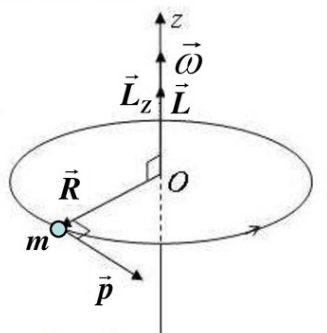
\includegraphics[width=0.5\linewidth]{pic/mip}
		\caption{}
		\label{mip}
	\end{figure}
	
	\item Сформулируйте методику измерений, используемую в лабораторной работе, и опишите лабораторную установку.
	
	Перед началом проведения эксперимента необходио найти центр масс маятника. После измерения маятник вешается на кронштейн и отклоняется на 5 градусов. Измеряется 10 полных колебаний. 
	
	Конструкция оборотного маятника представлена на
	рис. \ref{1}. На стержне 1 закреплены два диска – D 1 и D 2 . Маятник может быть подвешен на кронштейне к легкой
	призме, трение в которой пренебрежимо мало.
	
	\item Сформулируйте теорему Штейнера.
	
	момент инерции $I$ тела относительно произвольной неподвижной оси равен сумме момента инерции этого тела $I_c$ относительно параллельной ей оси, проходящей через центр масс тела, и произведения массы тела $m$ на квадрат расстояния $d$ между осями (рис. \ref{stein})
	
	\begin{equation}
	I = I_c + md^2
	\end{equation}
	
	\begin{figure}[h!]
		\centering
		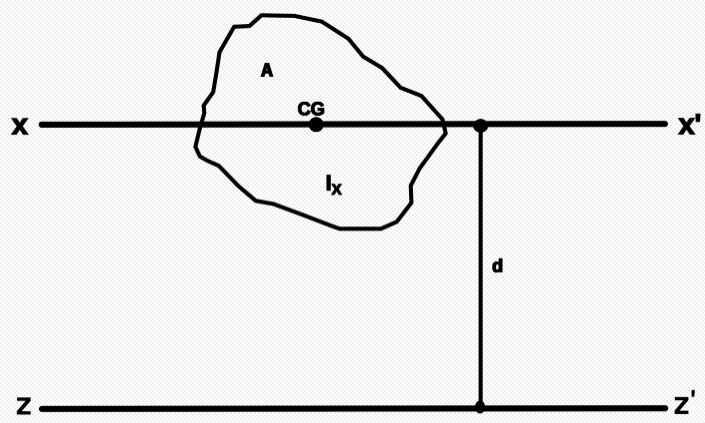
\includegraphics[width=0.5\linewidth]{pic/stein}
		\caption{}
		\label{stein}
	\end{figure}
	
	
	\item Одинаковы или различны угловые и линейные ускорения и скорости различных точек маятника в фиксированный момент времени при его колебаниях.
	
	При вращении твердого тела относительно неподвижной оси все его точки движутся с одинаковыми угловыми скоростями и одинаковыми угловыми ускорениями. За положительное направление вращения обычно принимают направление против часовой стрелки.
	
	\item Какие законы используются для описания колебаний физического маятника?
	
	При небольших углах отклонения $\alpha$ физический маятник так же совершает гармонические колебания. Будем считать, что вес физического маятника приложен к его центру тяжести в точке $С$. Силой, которая возвращает маятник в положение равновесия, в данном случае будет составляющая силы тяжести – сила $F$.
	
	\begin{equation}
	F = -mg\sin(\alpha)
	\end{equation}
	
	Знак минус в правой части означает то, что сила $F$ направлена в сторону уменьшения угла $\alpha$. С учетом малости угла $\alpha$
	
	\begin{equation}
	F = -mg\alpha
	\end{equation}
	
	Для вывода закона движения математического и физического маятников используем основное уравнение динамики вращательного движения $ I = md^2 $ Момент силы: определить в явном виде нельзя. С учетом всех величин, входящих в исходное дифференциальное уравнение колебаний физического маятника имеет вид:
	
	\begin{equation}
	\dfrac{d^2\alpha}{dt^2} + \dfrac{mgL}{I}\alpha = 0
	\end{equation}
	
	\begin{equation}
	\omega = \sqrt{\dfrac{mgL}{I}};     T = 2\pi\sqrt{\dfrac{I}{mgL}}
	\end{equation}
	
	\item Напишите дифференциальное уравнение гармонических колебаний осциллятора и его решение и объясните физический смысл величин, входящих в это уравнение.
	
	Дифференциальное уравнение гармонических колебаний осциллятора:
	
	\begin{equation}
	\dfrac{dS}{dt} = -A\omega_0\sin(\omega_0t+\varphi) = A\omega_0\cos(\omega_0t+\varphi+\dfrac{\pi}{2})
	\end{equation}
	
	Фаза $\dfrac{dS}{dt}$ отличается от фазы $S$ на $\dfrac{\pi}{2}$
	--- опережает.
	
	\begin{equation}
	\dfrac{d^2S}{dt^2} = -A\omega_0^2\cos(\omega_0t+\varphi) = -\omega_0^2A\cos(\omega_0t+\varphi) = A\omega_0^2\cos(\omega_0t+\varphi+\pi)
	\label{5}
	\end{equation}
	
	Фаза $\dfrac{d^2S}{dt^2}$ отличается от фазы $S$ на $\pi$ --- опережает.
	
	Из уравнения (\ref{5})
	следует, что гармонически колеблющаяся
	величина $S(t)$ удовлетворяет
	дифференциальному уравнению
	
	\begin{equation}
	\dfrac{d^2S}{dt^2} = -S\omega_0^2 \Rightarrow \dfrac{d^2S}{dt^2} + S\omega_0^2 = 0
	\end{equation}
	
	– дифференциальное уравнение
	гармонического колебания.
	
	Общее решение диф. уравнения
	гармонического колебания имеет вид
	
	\begin{equation}
	S = A_1\sin(\omega t) + A_2\cos(\omega t)
	\end{equation}
	
	где $A_1
	, A_2$ – произвольные постоянные
	интегрирования, которые можно найти
	из начальных условий $t = 0$. 
	
	\item Покажите, что максимальные кинетическая и потенциальная энергии тела,
	колеблющегося по гармоническому закону, совпадают с его полной механической энергией.
	
	Потенциальная энергия при достижении амплитудного значения угла
	отклонения маятника равна:
	\begin{equation}
	W_{pm} = mgh_c = mgx_c(1-\cos\varphi_m) = 2mgx_c\sin^2\dfrac{\varphi_m}{2}
	\end{equation}
	где $h_c$ высота поднятия центра масс маятника при его максимальном отклонении от положения равновесия, $x_c$ – положение центра масс маятника
	относительно его точки подвеса, $\varphi_m$ аксимальный угол отклонения маятника от положения равновесия.
	
	При малых углах отклонения маятника (до 20°) максимальная потенциальная энергия равна:
	
	\begin{equation}
	W_{pm} \approx \dfrac{1}{2}mgx_c\varphi_m^2
	\end{equation}
	
	Максимальная кинетическая энергия физического маятника
	
	\begin{equation}
	W_{km} = \dfrac{I\omega_m^2}{2} = \dfrac{mgx_cT_0^2\omega_m^2}{8\pi^2}
	\end{equation}
	
	где момент инерции маятника выражен по формуле (3) через период его ко-
	лебаний. таким образом, закон сохранения полной механической энергии включает в себя максимальные кинематическую и потенциальную энергии
	
	\begin{equation}
	W = W_k + W_p = W_{km} = W_{pm} = const
	\end{equation}
	
	
\end{enumerate}

\begin{comment}
\begin{table}[h!]
	\caption{Описание пользовательских функций и модулей программы}
	\label{funcsnmodules}
\begin{tabularx}{300pt}{|m{2,3 cm}|m{1,95 cm}|m{3 cm}|m{3 cm}|m {2,3 cm}|}
	\cline{1-5}
	Имя модуля & Имя функции & Назначение & Параметры функции & Возращаемое значение функции \\

	\cline{1-5} 
	openFile.h & openfile    & Открытие файла & int \&wordsSize, std::string \&name & std::string* \\ 
	
	\cline{1-5} 
	countVC.h & countVC & Подсчёт количества гласных и согласных в тексте & const std::string *words, int wordsSize, int \&V, int \&C, int \&N & void \\ 

	\cline{1-5} 
	writeFile.h & writeFile & Запись изменённого текста в файл & std::string *words, unsigned int wordsSize, char opt = '6' & void \\ 

	\cline{1-5} 
	countWords.h & countWords & Подсчёт количества слов в файле (без учёта повторений)& int wordsSize, std::string nameOfFile & bool \\ 
	
	\cline{1-5} 
	sortVC.h & sortVC & Сортировка слов в файле по заданным параметрам & std::string *words, const int \&wordsSize, char \&opt & void \\ 
	
	\cline{1-5} 
	printFile.h & printFile & Вывод содержимого файла на экран & const std::string *words, const int \&wordsSize & void \\ 
	
	\cline{1-5} 
	calck.h & calck & Подсчёт коэффициента слова по его гласным и согласным & const double \&v, const double \&c, const char \&opt & double \\ 
	\cline{1-5} 
\end{tabularx} 
\end{table}
\end{comment}
\end{document}